A Real Time Operating System (RTOS), is an operating system that must be able to
deal with time and event sensitive activities. The RTOS is intended
to be \textit{predictable} and \textit{determinant}\cite{RTOSMantis}. These
systems are also designed to limit the amount of overhead that is required to
context switch between tasks. This is done my making many critical decisions
prior to runtime.

\subsection{Tasks}

There are three different types of tasks in the RTOS; system tasks, periodic tasks and round robin tasks. These tasks are ordered in decreasing priority levels.

\begin{description}
    \item[System Tasks]
    System tasks are of the highest priority. If a system task is
    scheduled to run, it will preempt any other task.

    \item[Periodic Tasks]
    Periodic tasks are the next level below system tasks---middle priority.
    These tasks are scheduled to run periodically based on time (clock cycles).
    Periodic tasks are declared at the beginning of the program. A \texttt{PPP}
    array is also declared. This array allots time to each task and also
    declares an order for the periodic tasks. A periodic task is not allowed to
    take more time than has been allotted.  If this occurs, it is called a
    timing violation, and the system halts.

    \item[Round Robin Tasks]
    The final level---low priority -- consists of the round robin tasks. Round robin (RR) tasks
    are executed in the \textit{idle} time between periodic tasks.  The kernel
    maintains a FIFO queue containing all of the round robin tasks. On each clock
    cycle, if the system is not attending to either a system or periodic task then
    the next RR task is removed from the queue and is run for exactly one tick
    after which it is returned to the end of the FIFO queue. On the next cycle, if
    the higher priority tasks have not regained control, then the proceeding RR
    task is removed from the queue and executed.  
\end{description}



\subsection{Events and Timeouts}

System and round robin tasks are capable of waiting for an event, a timeout, or
either. The reason that only system and round robin tasks are allowed to wait on events is that if a periodic task waits longer than its time allowance, a timing violation will occur. \\

\noindent{\bf Events}\\
Events are initiated at the beginning of the program. Tasks that wait for an event are placed on a queue. The first item in the queue will continue when another task \textit{signals} that event. All of the elements will be released from the queue if another task \textit{broadcasts} that event. \\

\noindent{\bf Timeouts}\\
The kernel maintains a variable \textit{now} indicating how many ticks have occurred since program instantiation. When a task waits a certain amount of time, it will return normal operation after n ticks have passed.





The RTOS used for this project was created by Scott Craig and Justin Tanner \cite{RTOSSJ}. This RTOS is written in a mixture of C and assembly and is primarily written to support periodic tasks.   






\subsection{Tasks for Hovercraft 1---The leader}
In this project, hovercraft 1 assumes the role of a leader. It will navigate the
environment and make decisions to traverse the environment. Those decisions are then relayed to the trailing hovercraft, hovercraft 2. As a result, the implementation of hovercraft 1 is quite complex. This section will explain the
breakdown of the tasks in the implementation of hovercraft 1.

\begin{lstlisting}[float=th,label=lst:h1ppp,
                   caption={\texttt{PPP} array and task creation for hovercraft 1}]
const unsigned char PPP[] = {FIRE, 4, LISTEN, 1, FIRE, 4, LISTEN, 1, FIRE, 4,
LISTEN, 1, MOTOR, 5, RADIO, 8};
    Task_Create((void*)(&motor_task),0, PERIODIC, MOTOR);
    Task_Create((void*)(&fire_sonar),0, PERIODIC, FIRE);
    Task_Create((void*)(&listen_sonar),0,PERIODIC, LISTEN);
    Task_Create((void*)(&sendRadio),0,PERIODIC, RADIO);
	Task_Create((void*)(&stopSystem), 0,SYSTEM, STOP); 
\end{lstlisting}
The \texttt{PPP} array of hovercraft 1 and the task creation for the 5 tasks are shown in listing \ref{lst:h1ppp}.
There are in total four tasks, the first six items in the PPP array are the
two sonar tasks that are responsible for triggering and listening
to the three sonars. The integration of the sonar and the RTOS is based on the report by Will
Logan, Cambria Hanson and Jason Kereluk \cite{autoB}. In listing \ref{lst:h1sonarfire}, the implementation of the
\texttt{FIRE} task uses the built-in \texttt{Task\_Next()} function to trigger
the three sonars one by one. First, the task will trigger the front sonar, then
it will give up the CPU and allow the listen task (as shown in listing
\ref{lst:h1sonarlisten}) to calculate the distance. When the distances are
stored in their respective variables, the \texttt{MOTOR} task will run. Within
the \texttt{MOTOR} task, it will decide what speed the two motors should spin.
The code for the \texttt{MOTOR} is shown in listing \ref{lst:h1motor}. After
this, the radio task reports to both the base station and the follower
hovercraft. Listing \ref{lst:h1radio} illustrates this code. In this radio task, a test is set up to see if
three send tasks are sent before an ack is received. If this happens then the
program exits.

\begin{lstlisting}[float=thp,label=lst:h1sonarfire,
                   caption={\texttt{FIRE} Task}]
void fire_sonar(void) {
	for(;;) {
		trigger_sonar(FRONT);
		Task_Next();
		trigger_sonar(RIGHT);
		Task_Next();
		trigger_sonar(LEFT);
		Task_Next();
	}
}
\end{lstlisting}

\begin{lstlisting}[label=lst:h1sonarlisten,float=tbh,
                   caption={\texttt{LISTEN} Task}]
void listen_sonar(void) {
	for(;;)	{
	    s_forward= read_distance();
	    Task_Next();
	    s_right = read_distance();
	    Task_Next();
	    s_left = read_distance();
	    Task_Next();
	}
}
\end{lstlisting}

\begin{lstlisting}[label=lst:h1motor,float=th,
                   caption={\texttt{MOTOR} Task}]
void motor_task(void) {
	for(;;) {
    	if(s_front < MIN_DISTANCE &&  s_left >MAX_DISTANCE) {
            r_dir= FORWARD;
            r_duty = 255;
            l_dir = BACKWARD;
            l_duty = 255;
   		} else if (s_front < MIN_DISTANCE && s_right>MAX_DISTANCE) {
            r_dir = BACKWARD;
            r_duty = 255;
            l_dir= FORWARD;
            l_duty = 255;					
    	} else if (s_left < MIN_DISTANCE && s_right > MAX_DISTNACE) {
            l_dir = FORWARD;
            l_duty = 255;
            r_duty = 0;
   	 	} else if (s_right<MIN_DISTANCE && s_left > MAX_DISTANCE) {
            r_dir = BACKWARD;
            r_duty = 255;
            l_duty = 0;
    	} else {
            Signal_Event(stop);
    	}
        setMotorDirection(&rightMotor,r_dir;
        setMotorDuty(&rightMotor, r_duty);
        setMotorDirection(&leftMotor,l_dir);
        setMotorDuty(&leftMotor, l_duty);
	}
}
\end{lstlisting}

\begin{lstlisting}[label=lst:h1radio, float=th, caption={\texttt{RADIO} Task}]

void
sendRadio(void){
    for(;;){
        sendMovements(r_duty,l_duty,r_dir,r_duty);
        reportToBase(r_speed,l_speed, s_forward, s_right, s_left);
        send ++;
        if(send == 3)
            Event_Signal(stop);
        
        Task_Next();
    }
}



\end{lstlisting}

The Gantt chart in figure \ref{gantt} represents the timing for the periodic
tasks for hovercraft 1.

%\begin{minipage}{6.5in}
        \begin{center}
        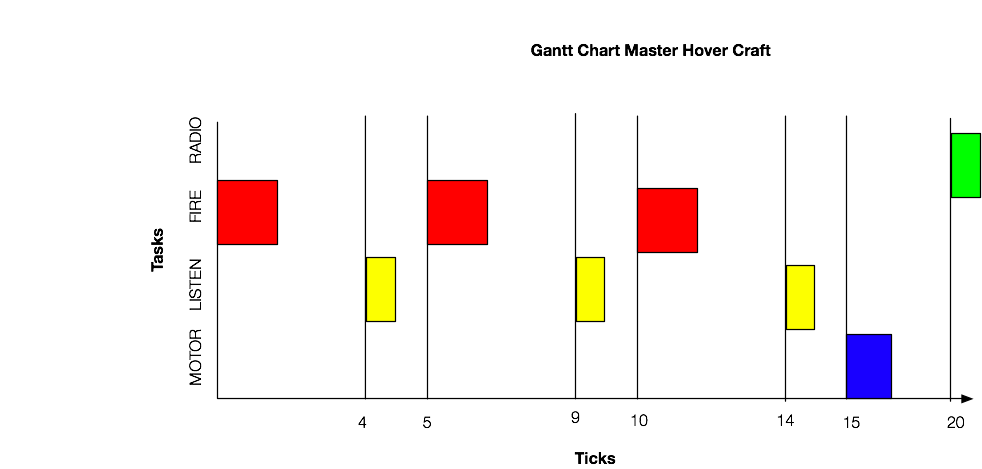
\includegraphics[width = 5.5in]{imageSources/Gantt.png}
        \captionof{figure}{Gantt chart for the master hovercraft}
        \label{gantt}
        \end{center}
%\end{minipage}

This hovercraft also has one system task. This task is responsible for
stopping the system if an error occurs and can be seen in listing \ref{lst:stop}. It attempts to stop the following
hovercraft before exiting. This system task waits for the \textit{stop} event
to be signaled.

\begin{lstlisting}[label=lst:stop, float=th, caption={\texttt{STOP} Task}]
void
stopSystem(void){
	Event_Wait(stop);
	sendMovements(0,0,FORWARD,FORWARD);
	exit(0);
}

\end{lstlisting}



\subsection{Tasks for Hovercraft 2 --- The Follower}

The second hovercraft has no periodic tasks. Most of the actions involved with
this hovercraft occur after events. As shown in in listing \ref{lst:h2setup}
there are three round robin tasks and a system task. The system task is very
similar to the system task in hovercraft 1. 


The motor and ack tasks from listing \ref{lst:h2motor} both wait on the same
event. This event occurs when a radio packet is received. This event is
broadcasted in the interrupt service routine (in listing \ref{isr} that is fired upon the detection
of an incoming packet.

The final task that belongs to this hovercraft is the pong task. This task is
part of the initial handshake. As noted in listing \ref{pong} this task does
not have a for loop, and only runs through once.

\begin{lstlisting}[label=lst:h2setup, float=th, caption={The Setup
calls for Hovercraft 2}]


        ack = Event_Init();
	pong = Event_Init();
	stop = Event_Init();

    
	Task_Create((void*)(&ack_task),0, RR, ACK);
        Task_Create((void*)(&up_motors),0, RR, MOTORS);
	Task_Creat((void*)(&pong_task),0,RR,PONG);
	Task_Create((void*)(&stopSystem), 0,SYSTEM, STOP);

 \end{lstlisting}



\begin{lstlisting}[label=lst:h2motor, float=th, caption={\texttt{MOTOR} Task}]

void
up_motors(void){

	for(;;){
		Event_Wait(ack);
                setMotorDuty(&rightMotor, rightMotorSpeed);	
                setMotorDuty(&leftMotor, leftMotorSpeed);
		setMotorDirection(&rightMotor, rightDirection);
		setMotorDirection(&leftMotor, leftDirection);
	}		
}	


void
ack_task(void){
	for(;;){
		Event_Wait(ack);
		sendACK;
	}
}

 \end{lstlisting}

\begin{lstlisting}[label=pong, float=th, caption={ISR that broadcasts Events}]
void
pong_task(void){


	Event_Wait(pong);
	sendPong();

}


 \end{lstlisting}



\begin{lstlisting}[label=isr, float=th, caption={ISR that broadcasts Events}]

ISR (INT4_vect)
{
    int i;
    
    PORTD ^= _BV(PORTD5);
    
    for (i = 0; i < PAYLOAD_BYTES; i++)
    {
        radio_buffer[i] = radio_get_byte();
    }
    
    // Figure out what type of packet this is.
    genericPacket_t *incomingPacket = (genericPacket_t *)radio_buffer;
    movePacket_t *theMovePacket;
    switch(incomingPacket->type) {
        case PING:
            pingReceived = true;
	    Signal_Event(pong);
            break;
        case MOVE:
            theMovePacket = (movePacket_t *) radio_buffer;
            rightMotorSpeed = theMovePacket->rightMotor;
            leftMotorSpeed  = theMovePacket->leftMotor;
	    rightDirection= theMovePacket-> rightDirection;
            leftDirection = theMovePacket -> leftDirection;
	    Event_Broadcast(ack);
            needSendAck = true;
            break;
        default:
            // ignore
            break;
    } 
\end{lstlisting}


\subsection{Tasks for the Base Station}

The final component to this project was a simple base station that would
report what was going on `out in the field'. This base station has one task
that is executed based on an event. This event is fired when a packet is
detected. 

The ISR is very similar to the isr in hovercraft 2 from listing \ref{isr}. It
uses event signal: \textit{Event\_Signal(radio\_event};

Listing \ref{print} shows the \textit{uart\_task} and
the \textit{printInfo(infoPacket\_t)} working together to display the
information to the screen.


\begin{lstlisting}[label=print, float=th, caption={ISR that broadcasts Events}]

void 
printInfo(infoPacket_t theInfo) 
{
    amount = sprintf(toPrint, SONAR_INFO_STRING, theInfo.frontSonar, theInfo.rightSonar,
                     theInfo.leftSonar);
    uart_write((uint8_t *)toPrint, amount);
    amount = sprintf(toPrint, MOTOR_INFO_STRING, theInfo.rightMotor, theInfo.leftMotor);
    uart_write((uint8_t *)toPrint, amount);
}


uart_task(void)
{
     for(;;)
    {
        Event_Wait(radio_event);
      	printInfo(*info);
        Task_Next();
    }
}

\end{lstlisting}
